\titleformat*{\chapter}{\centering\Huge\bfseries}
\chapter*{Appendix}
\addcontentsline{toc}{part}{Appendix}
\label{sec:appendix}

\titleformat{\chapter}[display]
{\filleft\bfseries}
{\filleft\chapnumfont\textcolor{chapnumcol}{\thechapter}}
{-2ex}
{\huge}

\chapter{Supplementary tables}
\newpage
\section{Additional information \cref{chapter:intro-heart}}
% Table generated by Excel2LaTeX from sheet 'GWAScatalogueHeart'
\begin{small}
\begin{longtable}{ll}
  \caption[\textbf{GWAS catalogue trait descriptions relating to cardiovascular diseases. }]{\textbf{GWAS catalogue trait descriptions relating to cardiovascular diseases. }Out of the \num{4148} studies in the \gls{gwas} catalogue (accessed 11.08.2017), \num{159} contain phenotype description related to cardiovascular diseases. For a summary of the studies conducted, they were broadly summarised into eight groups (Summary name). A graphical overview is shown in \cref{fig:gwas-heart}.}\\
  \toprule
  \endfirsthead
  \caption[]{\textbf{continued}} \\
  \toprule
 \endhead
 \bottomrule
 \endfoot
\bottomrule
\endlastfoot
    Summary name & GWAS catalogue trait \\
    \midrule
    \multirow{4}[1]{*}{Congenital heart disease} & Congenital heart disease \\
          & Congenital left-sided heart lesions (maternal effect) \\
          & Congenital left-sided heart lesions \\
          & Conotruncal heart defects \\
              \addlinespace[1.5ex]
    \multirow{8}[0]{*}{Coronary heart disease} & Coronary heart disease \\
          & Myocardial infarction \\
          & Myocardial infarction (early onset) \\
          & Coronary artery disease \\
       	  & Coronary heart disease event reduction in\\
       	  \addlinespace[-.5ex]
       	  & response to statin therapy (interaction) \\
          & Coronary restenosis \\
          & Myocardial infarction in coronary artery disease \\
              \addlinespace[1.5ex]
    		& Blood pressure \\
          & Hypertension \\
          & Systolic blood pressure \\
          & Diastolic blood pressure \\
          & Hypertension (young onset) \\
          & Systolic blood pressure in sickle cell anemia \\
          & Blood pressure (smoking interaction) \\
          & Blood pressure measurement (cold pressor test) \\
        Blood pressure & Blood pressure measurement (high sodium and \\
          \addlinespace[-.5ex]
          & potassium intervention) \\
          & Blood pressure measurement (low sodium intervention) \\
          & Blood pressure measurement (high sodium intervention) \\
          & Systolic blood pressure (alcohol consumption interaction) \\
          & Diastolic blood pressure (alcohol consumption interaction) \\
          & Mean arterial pressure (alcohol consumption interaction) \\
          & Pulse pressure (alcohol consumption interaction) \\
          & Pulse pressure in young-onset hypertension \\
          & Blood pressure (anthropometric measures interaction) \\
          & Blood pressure (age interaction) \\
          & Ejection fraction in Tripanosoma cruzi seropositivity \\
              \addlinespace[1.5ex]
    \multirow{18}[0]{*}{Electrocardiographic traits} & Atrial fibrillation \\
          & Echocardiographic traits \\
          & Atrial fibrillation/atrial flutter \\
          & QT interval \\
          & Electrocardiographic conduction measures \\
          & Atrioventricular conduction \\
          & QRS duration \\
          & Cardiac repolarization \\
          & QT interval (interaction) \\
          & P wave duration \\
          & PR segment \\
          & PR interval in Tripanosoma cruzi seropositivity \\
          & QT interval in Tripanosoma cruzi seropositivity \\
          & QRS duration in Tripanosoma cruzi seropositivity \\
          & Heart rate variability traits \\
          & PR interval \\
          & Resting heart rate \\
          & RR interval (heart rate) \\
              \addlinespace[1.5ex]
   			& Left ventricular mass \\
          & Cardiac structure and function \\
          & Cardiac muscle measurement \\
          Morphological traits & Cardiac hypertrophy \\
          & Dilated cardiomyopathy \\
          & Chagas cardiomyopathy in Tripanosoma \\
            \addlinespace[-.5ex]
          & cruzi seropositivity \\
              \addlinespace[1.5ex]
    \multirow{3}[0]{*}{Heart failure} & Heart failure \\
          & Sudden cardiac arrest \\
          & Mortality in heart failure \\
              \addlinespace[1.5ex]
    \multirow{2}[1]{*}{Others} & Cardiac Troponin-T levels \\
          & Cardiovascular disease risk factors \\
    \bottomrule
  \label{tab:gwas-studies}%
\end{longtable}%
\end{small}
%tab:gwas-studies

\newpage
\section{Additional results \cref{chapter:GWAS-3Dheart}}
% Table generated by Excel2LaTeX from sheet 'imputationQC'
\begin{table}[htbp]
  \centering
  \caption[\textbf{Number of SNPs after imputation, imputation QC and filtering for deviation from HWE and low MAF. }]{\textbf{Number of SNPs after imputation, imputation QC and filtering for deviation from HWE and low MAF. } Every batch was imputed independently (columns `SNPs after imputation'). \glspl{snp} that had an IMPUTE2 `info' metric of \(> 0.4\) in all of the batches were combined and subsequently filtered for \glspl{snp} deviating from Hardy-Weinberg equilibrium (\(p <0.001\)) and with low \gls{maf} (\(< 0.008\)), corresponding to a minor allele count of less than \num{20}. }
    \begin{tabular}{llllll}
    \toprule
    \multicolumn{1}{c}{\multirow{2}[4]{*}{Chr}} & \multicolumn{3}{c}{SNPs after Imputation} & \multicolumn{1}{c}{\multirow{2}[4]{*}{ INFO > 0.4}} & \multicolumn{1}{c}{\multirow{2}[4]{*}{HWE and MAF}} \\
\cmidrule{2-4}          & Sanger12 & Duke-NUS12 & Duke-NUS3 &       &  \\
    \midrule
    \num{1} & \num{3196692} & \num{3197145} & \num{3196563} & \num{1251157} & \num{719882} \\
    \num{2} & \num{3515670} & \num{3515861} & \num{3515602} & \num{1360182} & \num{780152} \\
    \num{3} & \num{2941265} & \num{2941468} & \num{2941223} & \num{1156243} & \num{665038} \\
    \num{4} & \num{2900679} & \num{2900786} & \num{2900634} & \num{1154742} & \num{684602} \\
    \num{5} & \num{2688219} & \num{2688348} & \num{2688174} & \num{1049671} & \num{606951} \\
    \num{6} & \num{2581500} & \num{2581851} & \num{2581410} & \num{1058844} & \num{635257} \\
    \num{7} & \num{2359370} & \num{2359598} & \num{2359319} & \num{932726} & \num{551744} \\
    \num{8} & \num{2323181} & \num{2323290} & \num{2323144} & \num{890407} & \num{514803} \\
    \num{9} & \num{1752242} & \num{1752363} & \num{1752199} & \num{698510} & \num{398777} \\
    \num{10} & \num{2003743} & \num{2003881} & \num{2003694} & \num{812616} & \num{474686} \\
    \num{11} & \num{2013331} & \num{2013535} & \num{2013273} & \num{794587} & \num{481479} \\
    \num{12} & \num{1947915} & \num{1948107} & \num{1947865} & \num{767854} & \num{452193} \\
    \num{13} & \num{1458325} & \num{1458401} & \num{1458308} & \num{590863} & \num{348525} \\
    \num{14} & \num{1333919} & \num{1333973} & \num{1333901} & \num{524391} & \num{309825} \\
    \num{15} & \num{1194294} & \num{1194406} & \num{1194264} & \num{458617} & \num{266813} \\
    \num{16} & \num{1289127} & \num{1289335} & \num{1289074} & \num{497688} & \num{286620} \\
    \num{17} & \num{1118587} & \num{1118772} & \num{1118528} & \num{434724} & \num{252227} \\
    \num{18} & \num{1153963} & \num{1154034} & \num{1153942} & \num{457454} & \num{268986} \\
    \num{19} & \num{877689} & \num{877866} & \num{877645} & \num{361419} & \num{222264} \\
    \num{20} & \num{912602} & \num{912721} & \num{912574} & \num{357156} & \num{210128} \\
    \num{21} & \num{546390} & \num{546414} & \num{546381} & \num{216911} & \num{131079} \\
    \num{22} & \num{531437} & \num{531528} & \num{531416} & \num{215547} & \num{129771} \\
    \midrule
    genome & \num{42989377} & \num{42993178} & \num{42988308} & \num{16042309} & \num{9391802} \\
    \bottomrule
    \end{tabular}%
  \label{tab:imputationQC}%
\end{table}%


\chapter{Supplementary Figures}
\newpage
\section{Additional results \cref{chapter:limmbo}}
\begin{figure}[hbtp]
	\centering
	\includegraphics[trim = 0mm 0mm 0mm 0mm, clip, width=\textwidth]{Supplement/Figures/powerAll.pdf}
		\caption[\textbf{All parameter combinations of power comparison for mvLMM and uvLMMs of high-dimensional phenotypes.}]{\textbf{All parameter combinations of power comparison for mvLMM and uvLMMs of high-dimensional phenotypes.} Each panels show the influence of one simulation parameter on the power to detect the causal \glspl{snp}.} 
	 	\label{fig:power-all}
\end{figure}

\newpage
\section{Additional results \cref{chapter:yeast}}
\begin{figure}[hbtp]
	\centering
	\includegraphics[trim = 0mm 0mm 0mm 0mm, clip, width=\textwidth]{Chapter3/Figures/manhattan-singletrait.pdf}
	\caption[\textbf{Manhattan plot of traits with strong single-trait associations.}]{\textbf{Manhattan plot of traits with strong single-trait associations.} Single-trait GWAS of A. magnesium sulfate and B. hydroquinone. The loci marked with a grey star are only found for these two traits and cannot be detected in the \gls{mtgwas} (\cref{fig:GWAS-yeast}), pointing to purely single-trait association that is burdened by the multi-trait testing based on \num{41} degrees of freedom. The  p-values were adjusted for multiple testing by the effective number of tests (\(M_\text{eff} = 33\)). The significance line is drawn at the empirical \(\text{FDR}_{\text{stGWAS}} =8.6 \times 10^{-6}\).}
 	\label{fig:stGWAS-yeast}
\end{figure}

\newpage
\section{Additional results \cref{chapter:DimReduction}}
\begin{figure}[hbtp]
	\centering
	\includegraphics[trim = 0mm 0mm 0mm 0mm, clip, width=0.65\textwidth]{Supplement/Figures/distributionAll-DimRed.pdf}
	\caption[\textbf{Additional scatterplots for visual assessment of low-dimensional components derived from left-ventricular wall thickness. }]{\textbf{Additional scatterplots for visual assessment of low-dimensional components derived from left-ventricular wall thickness. }Pairwise scatter plots of the components (lower triangle) and density plots (upper triangle) are depicted. The diagonal of each plot shows the distribution of the respective component. Row and column labels specify the rank of the component out of the \num{100} low-dimensional components. Before plotting, each component was mean-centred and divided by its standard deviation in order to have comparable axis dimensions. Given the normalised scale of the data, and the purpose of qualitative comparison, axis ticks were omitted for a cleaner visualisation. }
	 	\label{fig:distributionAll-DimRed}
\end{figure}

\newpage
\section{Additional results \cref{chapter:GWAS-3Dheart}}
\begin{figure}[hbtp]
	\centering
	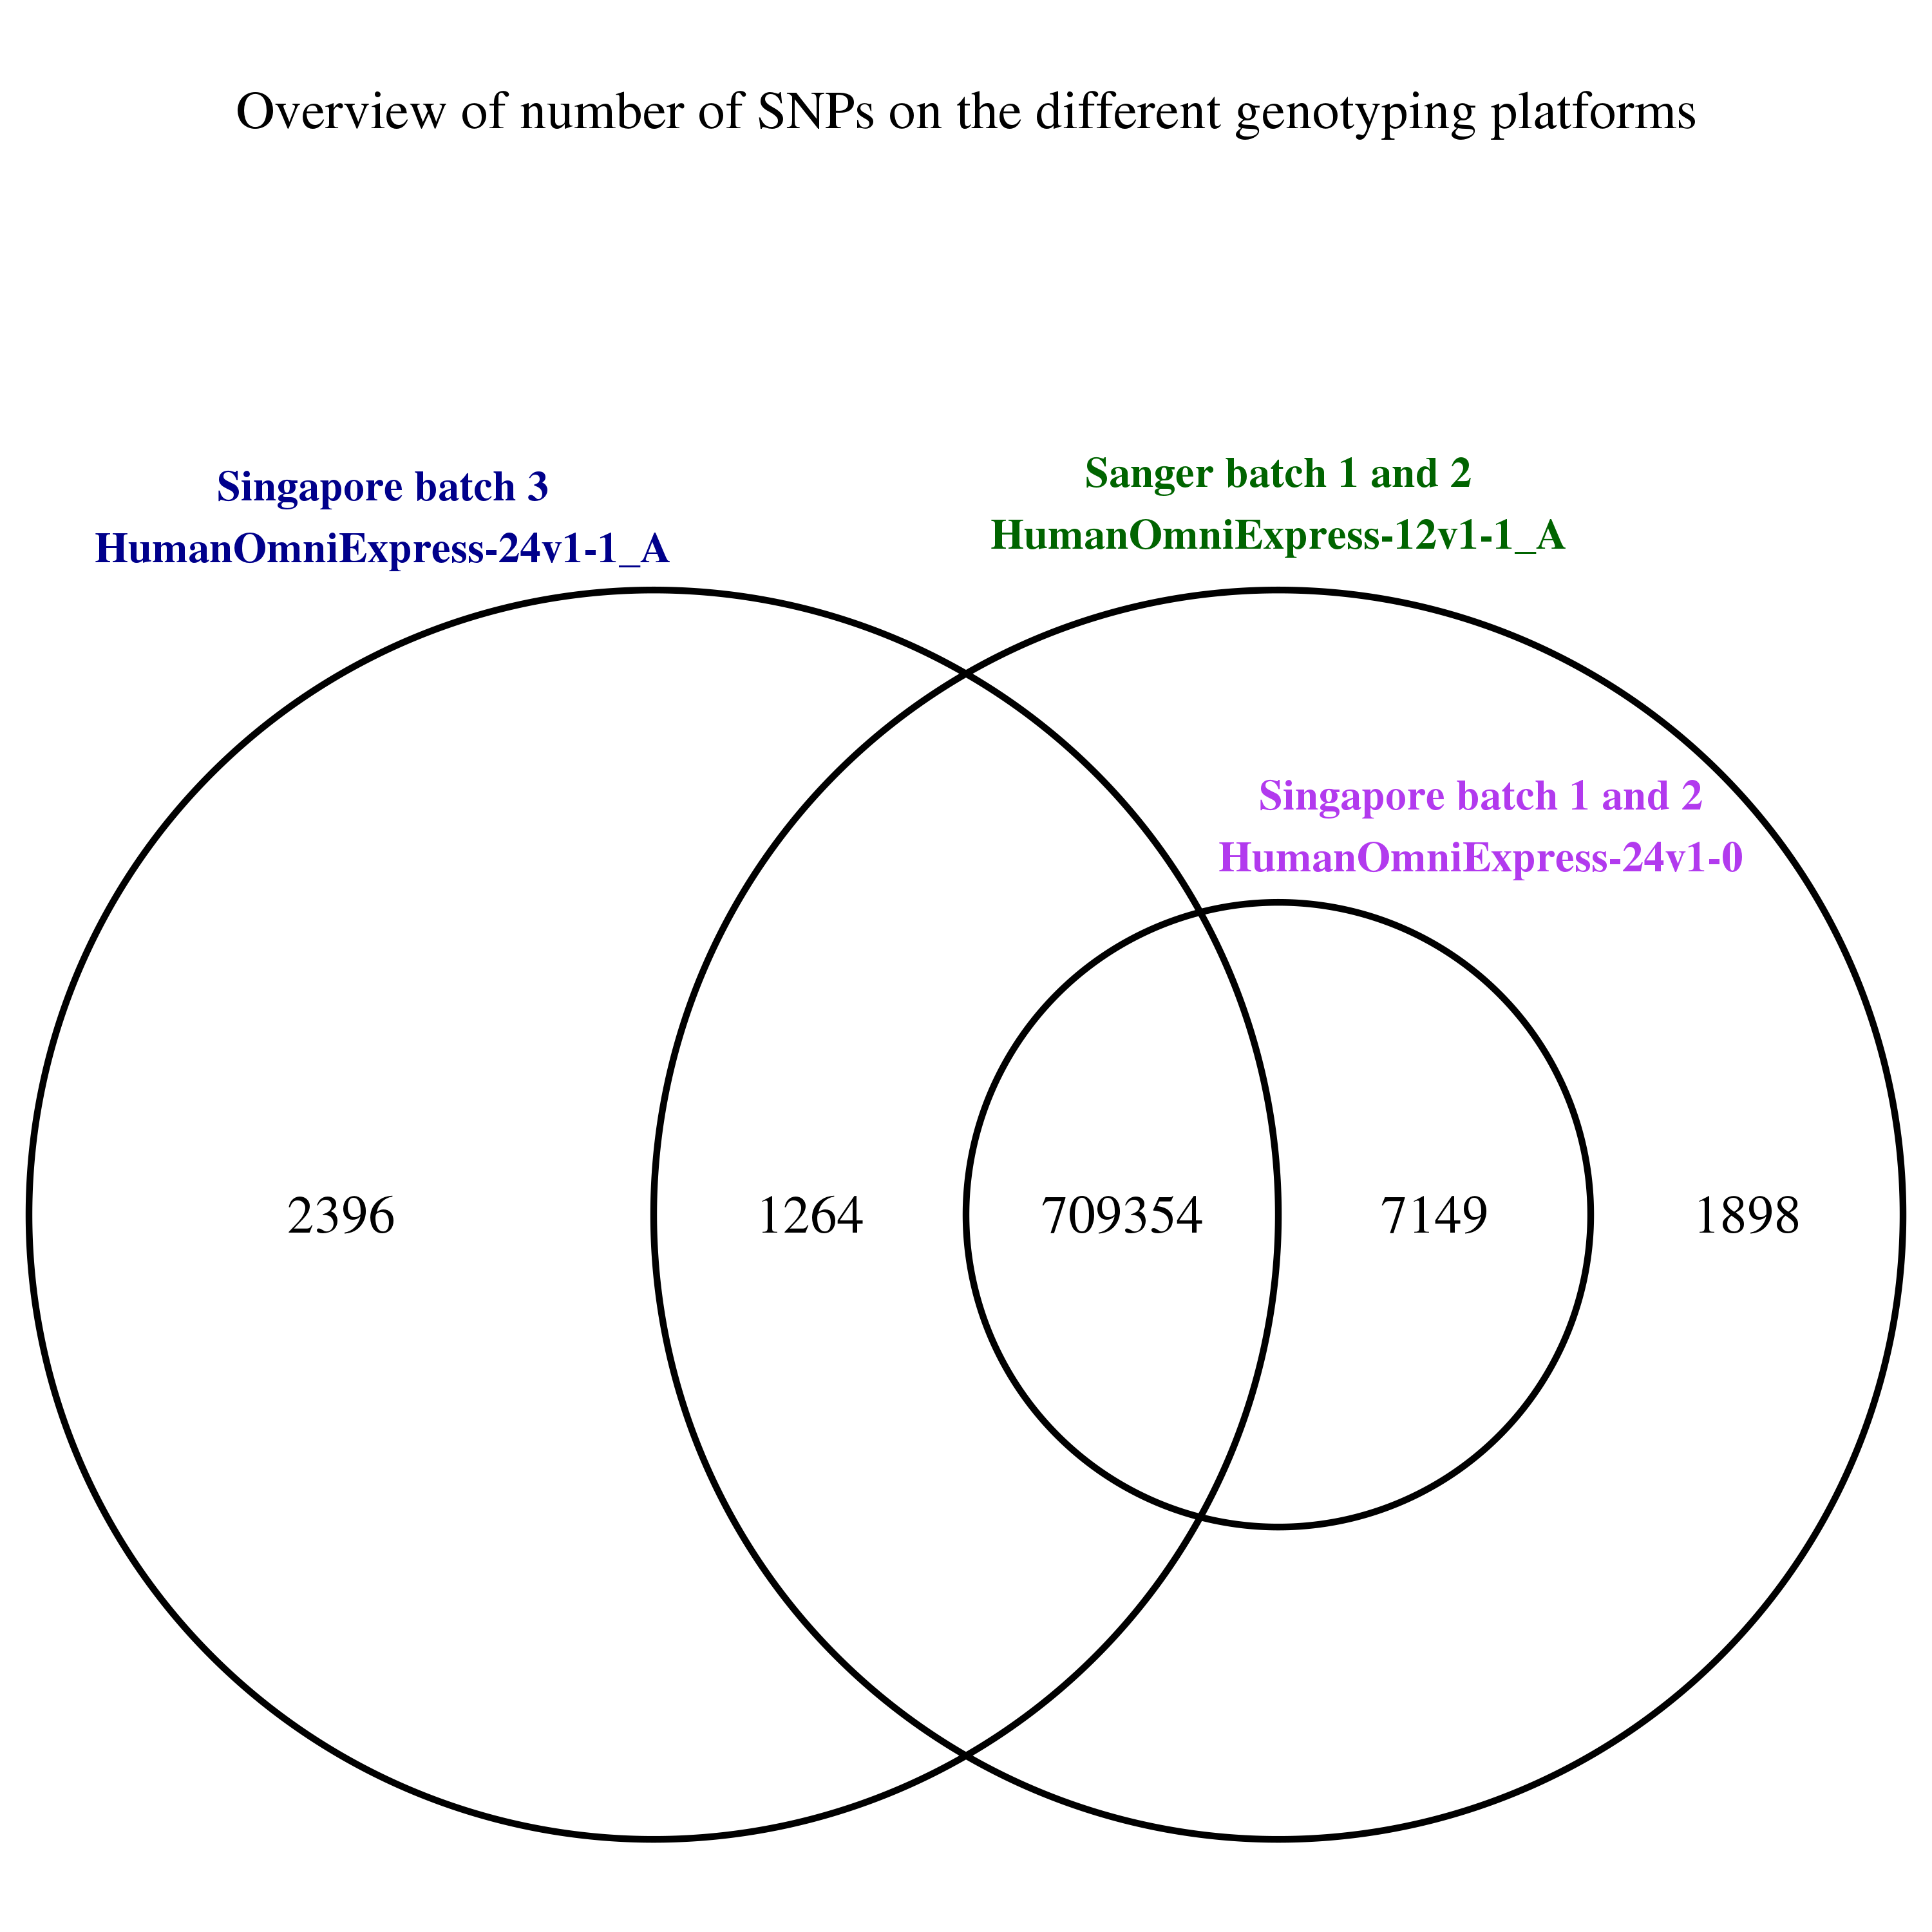
\includegraphics[trim = 0mm 0mm 0mm 20mm, clip, width=0.9\textwidth]{Supplement/Figures/Venn_genotyping_batches.pdf}
	\caption[\textbf{Number of DNA probes on the different genotyping chips and their overlap.}]{\textbf{Number of DNA probes on the different genotyping chips and their overlap.} For the genotyping of the individuals in the Digital Heart project three different Illumina HumanOmniExpress genotyping chips were used (24v1-1\_A, 12v1-1\_A, 24v1-0), differing in the number of probes on the chip (numbers inside Venn diagram) and the number of samples that can be genotyped (12 and 24; indicated in name of chip).}
 	\label{fig:probeoverlap}
\end{figure}

\begin{figure}[hbtp]
	\centering
	\includegraphics[trim = 0mm 0mm 0mm 0mm, clip, width=\textwidth]{Supplement/Figures/SampleQC.pdf}
	\caption[\textbf{Genotyping quality control per sample.}]{\textbf{Genotyping quality control per sample.} A. Sanger12. B. Duke-NUS12. C. Duke-NUS3. Supplementary plots for genotyping \gls{qc} described in \cref{subsection:genotypes}.}
 	\label{fig:sampleQC}
\end{figure}

\begin{figure}[hbtp]
	\centering
	\includegraphics[trim = 0mm 0mm 0mm 0mm, clip, width=\textwidth]{Supplement/Figures/SNPQC.pdf}
	\caption[\textbf{Genotyping quality control per SNP.}]{\textbf{Genotyping quality control per SNP.} A. Sanger12. B. Duke-NUS12. C. Duke-NUS3. Supplementary plots for genotyping \gls{qc} described in \cref{subsection:genotypes}.}
 	\label{fig:SNPQC}
 	\end{figure}

\begin{figure}[hbtp]
	\centering
	\includegraphics[trim = 0mm 0mm 0mm 0mm, clip,  width=\textwidth]{Supplement/Figures/kinshipQC.pdf}
	\caption[\textbf{Ethnicity of samples within the Digitial Heart project. }]{\textbf{Ethnicity of samples within the Digital Heart project.} A. Sanger12. B. Duke-NUS12. C. Duke-NUS3. \gls{pca} was conducted on the \gls{snp} genotypes of the samples within the Digital Heart project (gencall) and genotypes of four greater ethnicities of the HapMap project (black: African, orange:Mexican/Native American, grey: European, yellow: Asian) \citep{HapMap2005,HapMap2007}. The clustering of the samples based on the first and second principal components are depicted. Red dotted lines indicate borders considered to separate ancestries: 1. European, 2: African, 3: Mexican/Native American, 4. Asian, 5: Mixed ancestry. Gencall samples within the first group were used in \cref{chapter:GWAS-3Dheart,chapter:GWAS-FD}.  A description of the analysis is described in \cref{subsection:genotypes}.}
 	\label{fig:kinshipQC}
\end{figure}

\begin{figure}[hbtp]
	\centering
	\includegraphics[trim = 0mm 0mm 0mm 0mm, clip, width=0.65\textwidth]{Supplement/Figures/manhattan-all.pdf}
	\caption[\textbf{Manhattan plots for GWAS on stable components from a single dimensionality reduction method. }]{\textbf{Manhattan plots for GWAS on stable components from a single dimensionality reduction method. }The five stable components derived from Laplacian Eigenmaps (A), four from Isomap (B) and ten from \gls{pca} (C) were used as the response variables in three independent any effect \gls{mtgwas}. Their p-values were adjusted for the effective number of test conducted, estimated via \cref{eq:meff} based on the correlation across their components (\cref{fig:dimRed-correlation}): \(M_{eff}=2.04\). The horizontal grey line is drawn at the level of genome-wide significance: \(p = 5 \times 10^{-8}\). Only the locus on chromosome 1 which was detected in the combined analyses (\cref{fig:manhattan-heart}) could also be detected via components from Laplacian Eigenmaps alone. } 
	 	\label{fig:manhattan-3Dheart-single}
\end{figure}

\newpage
\section{Additional results \cref{chapter:GWAS-FD}}
\begin{figure}[hbtp]
	\centering
	\includegraphics[trim = 0mm 0mm 0mm 0mm, clip, width=0.65\textwidth]{Supplement/Figures/manhattan-FD-single.pdf}
	\caption[\textbf{Manhattan plot of  two single-trait GWAS on left ventricular trabeculation. }]{\textbf{Manhattan plot of two single-trait GWAS on left ventricular trabeculation } The maximal apical (A) and basal \gls{fd} (B) were used as the response variable in a \gls{stgwas}.  Their p-values were adjusted for the effective number of test conducted, estimated via \cref{eq:meff} based on their correlation: \(M_{eff}=1.86\). The p-values of all genome-wide \glspl{snp} are depicted. The horizontal grey line is drawn at the level of genome-wide significance: \(p = 5 \times 10^{-8}\).} 
	 	\label{fig:manhattan-FD-single}
\end{figure}



\chapter{Derivations}
\label{section:simulating-G}
The following section describes the derivation of the simulation scheme for the infinitesimal genetic effects in \cref{section:phenotype-simulation}.
A suitable model for simulating the infinitesimal genetic effect \(\mat{G} \inR N P\) with known \(N \times N\) sample (row) covariance is a matrix-normally distributed random variable, defined by its mean \(\mat{M} \inR N P\), its row covariance \(\mat{D} \inR N N\) and its column covariance \(\mat{C} \inR P P\): 
%
\begin{equation}
\mat{G} \sim \matrixnormal N P M D C.
\label{eq:mvn}
\end{equation}
%
With the \(N \times N\) sample-by-sample covariance captured in \(R\) and  \(\mat{M}=0\), the component of \tmat{G} which has to be simulated is the trait-by-trait covariance \tmat{C}:
%
\begin{equation}
\mat{G} \sim  \matrixnormal N P 0 R C
\label{eq:G-mvn}
\end{equation}
%
The structure of \tmat{C} depends on the design of the covariance effect. In order to simulate \tmat{C}, \tmat{G} is first expressed in terms of a multivariate normal distribution 
%
\begin{equation}
\text{vec}(\mat{G}) \sim \multinormal N P {\mat{0}} {\mat{C} \otimes \mat{R}}.
\end{equation}
%
With the Cholesky decomposition of \tmat{R} and \tmat{C} into  \(\mat{R}=\mat{BB}^T\) and \(\mat{C}=\mat{AA}^T\) 
%
\begin{equation}
\text{vec}(\mat{G}) \sim \multinormal N P {\mat{0}} {\mat{AA}^T  \otimes \mat{BB}^T},  
\end{equation}
%
which can be rearranged as 
%
\begin{equation}
\begin{aligned}
\text{vec}(\mat{G}) & \sim \multinormal N P {\mat{0}} {(\mat{A }\otimes \mat{B}) \mat{I} (\mat{A} \otimes\mat{B})^T)}. 
\end{aligned}
\end{equation}
\tmat{I} is the identity matrix.
 %
Using the property of a normally distributed random variable \tmat{Y} with mean \tmat{\mu} and covariance matrix \tmat{\Sigma}
%
\begin{equation}
\begin{aligned} 
w \mat{Y} \sim \normal {w\mat{\mu}}  {w\mat{\Sigma} w^T},
\end{aligned}
\end{equation}
%
we can let  \(\text{vec} (\mat{G}) =  (\mat{A} \otimes \mat{B}) \text{vec} (\mat{Y})\)  and \(\mat{Y} \sim \multinormal N P {\mat{0}} {\mat{I}}\) such that
%
\begin{equation}
\begin{aligned}
(\mat{A} \otimes\mat{B}) \text{vec} (\mat{Y})  \sim \multinormal N P {\mat{0}} {(\mat{A} \otimes \mat{B}) \mat{I} (\mat{A} \otimes \mat{B})^T}
\end{aligned}
\end{equation}
%
Using \citep{Horn1985}: Lemma 4.3.1, we get 
\begin{equation}
(\mat{A} \otimes \mat{B}) \text{vec}(\mat{Y}) = \text{vec}(\mat{BYA}^T) = \text{vec}(\mat{G}).
\label{eq:G-vec}
\end{equation}
%



